\documentclass[twoside,11pt]{article}

\usepackage{amsmath,amssymb,amsthm}
\usepackage{booktabs}
\usepackage{graphicx}
\usepackage{hyperref}
\usepackage[round]{natbib}

\newtheorem{proposition}{Proposition}

\title{semflow-dl: Edge-Level White-Box Causal Deep Learning with Monotonic I-Splines and Conformal Guarantees}
\author{Chatchawich Chaihong \\
Department of Interdisciplinary Engineering, Faculty of Engineering \\
Prince of Songkla University, Hat Yai, Songkhla, Thailand}
\date{November 22, 2026}

\begin{document}
\maketitle

\begin{abstract}
Flat interpretable machine learning models such as Explainable Boosting Machines (\texttt{EBM}) and post-hoc \texttt{XGBoost+SHAP} fail to propagate interventions through mediated causal pathways (\emph{mediator blocking}) and often violate domain monotonicity in sparse distribution tails. Conversely, classical Structural Equation Modeling (SEM) captures latent causal graphs but is limited to linear structural equations. We present \texttt{semflow-dl}, a pure-Rust edge-level white-box causal deep learning library with zero-copy Python bindings. By parameterizing structural DAG edges with Ramsay's monotonic I-Splines, ANOVA-purified 2D interactions, and split-conformal calibration, \texttt{semflow-dl} guarantees global $C^1$ monotonicity ($0.0\%$ violations), exact closed-form local causal elasticity via M-Spline derivatives, exact direct--indirect counterfactual decomposition under Pearl's $\mathrm{do}(\cdot)$ operator, and finite-sample coverage guarantees. Empirically, \texttt{semflow-dl} reduces causal intervention error by over $5\times$ compared to \texttt{EBM} and \texttt{XGBoost+SHAP} while consuming $2.4\times\text{--}2.9\times$ less peak memory.
\end{abstract}

\section{Introduction}
\label{sec:intro}

Interpretable machine learning in high-stakes scientific, medical, and engineering domains increasingly demands models that are simultaneously \emph{accurate}, \emph{mechanistically transparent}, and \emph{actionable under intervention}. In practice, practitioners face a sharp dichotomy between two dominant modeling paradigms:

\begin{enumerate}
  \item \textbf{Flat Black-Box and Glass-Box Predictors:} Gradient-boosted decision trees such as \texttt{XGBoost} \citep{chen2016xgboost} paired with post-hoc \texttt{SHAP} attributions \citep{lundberg2017unified}, as well as Generalized Additive Models (GAMs) such as Explainable Boosting Machines (\texttt{EBM}) \citep{lou2013accurate} and Neural Additive Models (\texttt{NAM}) \citep{agarwal2021neural}, treat all observed features as flat covariates in a single regression equation $y = f(\mathbf{x})$. When a dataset contains mediated causal pathways ($X \to M \to Y$) or noisy multi-indicator measurements, flat predictors suffer from \emph{mediator blocking}: holding $M$ fixed while perturbing $X$ zeros out the indirect causal pathway, severely underestimating the true intervention effect $\mathrm{do}(X + \Delta)$ and misallocating feature importance away from upstream root causes. Moreover, histogram- or tree-based shape functions frequently exhibit non-monotonic oscillations in sparsely populated tails, violating domain physics or clinical monotonicity priors.
  \item \textbf{Classical Structural Equation Modeling (SEM):} Covariance-based SEM \citep{bollen1989structural,rosseel2012lavaan} and Partial Least Squares SEM \citep{wold1982soft,dijkstra2015consistent} explicitly separate noisy measurement indicators from latent constructs and model directed causal graphs. However, classical SEM is predominantly restricted to linear structural equations, lacks native distribution-free uncertainty quantification, and cannot capture nonlinear saturation or convex acceleration regimes without manual polynomial specification.
\end{enumerate}

To bridge these two worlds, we introduce \texttt{semflow-dl}, an edge-level white-box causal deep learning framework implemented in pure Rust with zero-copy Python bindings. Rather than replacing structural equations with opaque node-level multilayer perceptrons, \texttt{semflow-dl} preserves the directed acyclic graph (DAG) of anchored latent constructs and equips each structural edge $(i, j)$ with an interpretable univariate operator---specifically Ramsay's monotonic I-Splines \citep{ramsay1988monotone} and ANOVA-purified 2D interactions \citep{lou2013accurate}. This design yields four key properties: (i) guaranteed global $C^1$ monotonicity with closed-form local causal elasticity $\phi'_{ij}(z)$ via M-Spline derivatives; (ii) exact counterfactual decomposition of Pearl's $\mathrm{do}(\eta_i + \Delta)$ into direct and indirect effects \citep{pearl2009causality}; (iii) finite-sample, distribution-free prediction intervals via split-conformal calibration \citep{lei2018distribution}; and (iv) CPU-only training requiring 246\,ms on $10^4$ observations and 5.9\,s on $10^5$ observations within 87\,MB of peak RAM (a $2.4\times\text{--}2.9\times$ memory reduction compared to EBM and XGBoost+SHAP).

\section{Related Work}
\label{sec:related}

\paragraph{Glass-Box Additive Models and KANs.}
Explainable Boosting Machines (\texttt{EBM}) \citep{lou2013accurate} and Neural Additive Models (\texttt{NAM}) \citep{agarwal2021neural} learn univariate shape functions $f_j(x_j)$ and purified pairwise interactions, while Kolmogorov--Arnold Networks (\texttt{KAN}) \citep{liu2024kan} place learnable B-spline activations on network edges. Unlike \texttt{EBM} and \texttt{NAM}, which remain flat regressors without latent measurement layers or causal DAG propagation, and unlike \texttt{KAN}, which composes deep dense layers of splines without structural identification or guaranteed monotonicity, \texttt{semflow-dl} binds each edge spline directly to an identified latent causal graph with exact M-spline elasticity and $\mathrm{do}(\cdot)$ semantics.

\paragraph{Nonlinear and Causal SEM.}
Prior extensions of nonlinear SEM rely on latent interaction products \citep{klein2000maximum} or deep neural network encoders \citep{pearl2009causality} that sacrifice edge-level interpretability and monotonicity guarantees. \texttt{semflow-dl} complements classical linear SEM engines such as \texttt{lavaan} \citep{rosseel2012lavaan}, \texttt{semopy} \citep{igolkina2020semopy}, and \texttt{semflow} by providing a modular external plugin that shares the same \texttt{lavaan+}-compatible formula DSL and zero-copy Rust linear algebra foundation.

\section{Methodology: Edge-Level White-Box Causal Deep Learning}
\label{sec:methodology}

To resolve the tension between opaque black-box predictors (\texttt{XGBoost}+SHAP) and flat glass-box additive models (EBM, NAM) that suffer from mediator blocking and measurement attenuation, we introduce \texttt{semflow-dl}, an edge-level white-box structural causal architecture.

\subsection{Anchored Latent Measurement and Edge-Level Structural Graph}
Let $\mathcal{G} = (\mathcal{V}, \mathcal{E})$ be a directed acyclic graph (DAG) over $K$ latent constructs $\boldsymbol{\eta} = (\eta_1, \dots, \eta_K)^\top$, ordered topologically such that $(i, j) \in \mathcal{E} \implies i < j$. Each latent variable $\eta_k$ is observed through a block of noisy indicators $\mathbf{x}_k \in \mathbb{R}^{m_k}$:
\begin{equation}
  \mathbf{x}_k = \boldsymbol{\lambda}_k \eta_k + \boldsymbol{\delta}_k,
  \qquad \mathbb{E}[\eta_k] = 0, \quad \operatorname{Var}(\eta_k) = 1, \quad \lambda_{k,1} > 0,
  \label{eq:anchored-measurement}
\end{equation}
where the unit-variance and positive-first-loading constraints serve as an \emph{identification anchor}, eliminating sign and scale indeterminacy during nonlinear optimization.

Rather than passing all parent variables into an opaque node-level multilayer perceptron, \texttt{semflow-dl} assigns a transparent, univariate operator $\phi_{ij}: \mathbb{R} \to \mathbb{R}$ to each structural edge $(i, j) \in \mathcal{E}$:
\begin{equation}
  \eta_j = b_j + \sum_{i \in \mathrm{Pa}(j)} \phi_{ij}(\eta_i) + \zeta_j,
  \qquad \mathbb{E}\big[\phi_{ij}(\eta_i)\big] = 0,
  \label{eq:edge-structural}
\end{equation}
where $\zeta_j$ is an exogenous structural disturbance with $\mathbb{E}[\zeta_j \mid \mathrm{Pa}(j)] = 0$.

\subsection{Monotonic I-Spline Edge Operators and Exact Local Elasticity}
For edges governed by domain monotonicity (e.g., physical degradation or clinical risk progression), we parameterize $\phi_{ij}$ using Ramsay's integrated B-splines (I-Splines) \citep{ramsay1988monotone}. Given a clamped knot sequence $t_0 \le \dots \le t_{B+k}$ of order $k \ge 3$ constructed from empirical quantiles of $\eta_i$, the $b$-th I-Spline basis function is defined as the integral of the corresponding nonnegative M-Spline $M_b(z) \ge 0$:
\begin{equation}
  I_b(z) = \int_{t_{\min}}^{z} M_b(u)\,du \in [0, 1], \qquad \frac{d}{dz} I_b(z) = M_b(z) \ge 0.
\end{equation}
We define the \emph{Monotonic I-Spline Edge Operator} with prescribed direction $s_{ij} \in \{+1, -1\}$ as:
\begin{equation}
  \phi_{ij}^{\mathrm{mono}}(z; \boldsymbol{\alpha}_{ij})
  = s_{ij}\!\left(\operatorname{softplus}(\alpha_{ij,0})\,z + \sum_{b=1}^{B} \operatorname{softplus}(\alpha_{ij,b})\,I_b(z)\right) - \mu_{ij},
  \label{eq:ispline-edge}
\end{equation}
where $\operatorname{softplus}(a) = \ln(1 + e^a)$, $\boldsymbol{\alpha}_{ij} \in \mathbb{R}^{B+1}$ are unconstrained learnable parameters, and $\mu_{ij} = \frac{1}{N}\sum_{n=1}^N \tilde{\phi}_{ij}(\eta_{i,n})$ enforces zero-mean centering. Each endogenous node $j$ is trained by minimizing the regularized empirical risk:
\begin{equation}
  \mathcal{L}_j(\boldsymbol{\theta}_j) = \frac{1}{N}\sum_{n=1}^{N}\big(\eta_{j,n} - \hat{\eta}_{j,n}\big)^2
  + \lambda_{\mathrm{smooth}} \sum_{i \in \mathrm{Pa}(j)} \sum_{b=1}^{B} \big(\operatorname{softplus}(\alpha_{ij,b})\big)^2.
  \label{eq:node-loss}
\end{equation}

\begin{proposition}[Global Smooth Monotonicity and Exact Local Causal Elasticity]
\label{prop:monotonicity}
For any finite parameter vector $\boldsymbol{\alpha}_{ij} \in \mathbb{R}^{B+1}$, knot order $k \ge 3$, and direction $s_{ij} \in \{+1, -1\}$, the edge operator $\phi_{ij}^{\mathrm{mono}}(z; \boldsymbol{\alpha}_{ij})$ in \eqref{eq:ispline-edge} is continuously differentiable ($C^1$-smooth) everywhere on $\mathbb{R}$, strictly monotonic in direction $s_{ij}$ across the entire real line (including out-of-range tails), and admits a closed-form local causal elasticity:
\begin{equation}
  \phi'_{ij}(z) = \frac{\partial \phi_{ij}^{\mathrm{mono}}(z)}{\partial z}
  = s_{ij}\!\left(\operatorname{softplus}(\alpha_{ij,0}) + \sum_{b=1}^{B}\operatorname{softplus}(\alpha_{ij,b})\,M_b(z)\right),
  \qquad s_{ij}\,\phi'_{ij}(z) > 0 \;\; \forall z \in \mathbb{R}.
\end{equation}
\end{proposition}

\begin{proof}
For order $k \ge 3$, each M-Spline $M_b(z)$ is a piecewise polynomial of degree $k - 1 \ge 2$ that is continuous on $\mathbb{R}$ and satisfies $M_b(z) \ge 0$ everywhere with compact support $[t_{\min}, t_{\max}]$. By the Fundamental Theorem of Calculus, $I_b(z) = \int_{t_{\min}}^z M_b(u)\,du$ is continuously differentiable with $I'_b(z) = M_b(z)$ on $\mathbb{R}$ (with $M_b(z) = 0$ outside $[t_{\min}, t_{\max}]$). Differentiating \eqref{eq:ispline-edge} term-by-term yields the stated expression for $\phi'_{ij}(z)$. Because $\operatorname{softplus}(a) = \ln(1 + e^a) > 0$ strictly for all finite $a \in \mathbb{R}$ and $M_b(z) \ge 0$, we obtain:
\[
  s_{ij}\,\phi'_{ij}(z) = \operatorname{softplus}(\alpha_{ij,0}) + \sum_{b=1}^{B}\operatorname{softplus}(\alpha_{ij,b})\,M_b(z) \ge \operatorname{softplus}(\alpha_{ij,0}) > 0 \qquad \forall z \in \mathbb{R}.
\]
Thus $\phi_{ij}^{\mathrm{mono}}$ is strictly monotonic everywhere with zero monotonicity violations, even under extreme tail extrapolation.
\end{proof}

\subsection{Exact Structural Intervention and Mediation Decomposition}
Given a fitted DAG $\mathcal{G}$, \texttt{semflow-dl} evaluates Pearl's counterfactual shift intervention $\mathrm{do}(\eta_i \leftarrow \eta_i + \Delta)$ via three exact steps:
\begin{enumerate}
  \item \textbf{Abduction:} Recover individual-level structural residuals $\hat{\zeta}_{k,n} = \eta_{k,n} - \big(b_k + \sum_{u \in \mathrm{Pa}(k)} \phi_{uk}(\eta_{u,n})\big)$ for all endogenous $k$.
  \item \textbf{Action:} Mutilate incoming edges to node $i$ and set $\eta_{i,n}^{\mathrm{cf}} = \eta_{i,n} + \Delta$.
  \item \textbf{Prediction:} Propagate sequentially along the topological order of $\mathcal{G}$:
  \begin{equation}
    \eta_{k,n}^{\mathrm{cf}} = b_k + \hat{\zeta}_{k,n} + \sum_{u \in \mathrm{Pa}(k)} \phi_{uk}(\eta_{u,n}^{\mathrm{cf}}), \qquad \forall k \neq i.
  \end{equation}
\end{enumerate}

\begin{proposition}[Exact Nonlinear Direct--Indirect Decomposition]
\label{prop:mediation}
Under the additive edge-level structural model \eqref{eq:edge-structural} on a correctly specified DAG $\mathcal{G}$, the average total treatment effect $\mathrm{ATE}_{\mathrm{Total}}(\Delta) = \frac{1}{N}\sum_{n=1}^N (\eta_{j,n}^{\mathrm{cf}} - \eta_{j,n})$ on target node $j$ under $\mathrm{do}(\eta_i \leftarrow \eta_i + \Delta)$ decomposes without approximation error into the exact sum of the direct effect and the mediated indirect effect:
\begin{equation}
  \mathrm{ATE}_{\mathrm{Total}}(\Delta)
  = \underbrace{\frac{1}{N}\sum_{n=1}^{N}\Big[\phi_{ij}(\eta_{i,n} + \Delta) - \phi_{ij}(\eta_{i,n})\Big]}_{\mathrm{ADE}_{\mathrm{Direct}}(\Delta)}
  + \underbrace{\frac{1}{N}\sum_{n=1}^{N}\sum_{m \in \mathrm{Pa}(j) \setminus \{i\}} \Big[\phi_{mj}(\eta_{m,n}^{\mathrm{cf}}) - \phi_{mj}(\eta_{m,n})\Big]}_{\mathrm{AIE}_{\mathrm{Indirect}}(\Delta)}.
\end{equation}
\end{proposition}

\begin{proof}
Subtracting $\eta_{j,n} = b_j + \hat{\zeta}_{j,n} + \sum_{u \in \mathrm{Pa}(j)} \phi_{uj}(\eta_{u,n})$ from $\eta_{j,n}^{\mathrm{cf}} = b_j + \hat{\zeta}_{j,n} + \sum_{u \in \mathrm{Pa}(j)} \phi_{uj}(\eta_{u,n}^{\mathrm{cf}})$ cancels both the intercept $b_j$ and the abducted disturbance $\hat{\zeta}_{j,n}$ identically for every sample $n$. Splitting $\mathrm{Pa}(j)$ into $\{i\}$ (if $(i, j) \in \mathcal{E}$) and $\mathrm{Pa}(j) \setminus \{i\}$, and substituting $\eta_{i,n}^{\mathrm{cf}} = \eta_{i,n} + \Delta$, yields the exact sample-wise identity. Averaging over $n = 1, \dots, N$ completes the proof. In contrast, any flat additive model $\hat{y} = \sum f_u(x_u)$ fixes $\eta_{m,n}^{\mathrm{cf}} \equiv \eta_{m,n}$ for all mediators $m$, forcing $\mathrm{AIE}_{\mathrm{Indirect}} \equiv 0$ (mediator blocking).
\end{proof}

\subsection{Distribution-Free Split-Conformal Calibration}
To quantify predictive uncertainty without Gaussian residual assumptions, we partition a held-out calibration set $\mathcal{D}_{\mathrm{cal}}$ of size $N_{\mathrm{cal}}$ and compute absolute nonconformity scores $R_m = |\eta_{j,m} - \hat{\eta}_{j,m}|$ for $m = 1, \dots, N_{\mathrm{cal}}$. Let $q_{1-\alpha}$ be the $\lceil (N_{\mathrm{cal}} + 1)(1 - \alpha) \rceil / N_{\mathrm{cal}}$ empirical quantile of $\{R_m\}_{m=1}^{N_{\mathrm{cal}}}$.

\begin{proposition}[Finite-Sample Conformal Coverage]
\label{prop:conformal}
Assume the calibration samples $\mathcal{D}_{\mathrm{cal}}$ and a new test point $(\mathbf{x}_{\mathrm{test}}, \eta_{j,\mathrm{test}})$ are exchangeable. Then, for any miscoverage level $\alpha \in (0, 1)$ and any underlying residual distribution, the prediction interval $\mathcal{C}_{1-\alpha}(\mathbf{x}_{\mathrm{test}}) = [\hat{\eta}_{j,\mathrm{test}} - q_{1-\alpha},\; \hat{\eta}_{j,\mathrm{test}} + q_{1-\alpha}]$ satisfies:
\begin{equation}
  \mathbb{P}\!\left(\eta_{j,\mathrm{test}} \in \mathcal{C}_{1-\alpha}(\mathbf{x}_{\mathrm{test}})\right) \ge 1 - \alpha.
\end{equation}
\end{proposition}

\begin{proof}
Because the measurement anchors and edge parameters $\hat{\boldsymbol{\theta}}$ are fixed prior to evaluating $\mathcal{D}_{\mathrm{cal}}$, the nonconformity scores $R_1, \dots, R_{N_{\mathrm{cal}}}, R_{\mathrm{test}}$ are exchangeable random variables. By the standard split-conformal rank lemma \citep{lei2018distribution}, the rank of $R_{\mathrm{test}}$ among $\{R_1, \dots, R_{N_{\mathrm{cal}}}, R_{\mathrm{test}}\}$ is uniformly distributed over $\{1, \dots, N_{\mathrm{cal}} + 1\}$ (breaking ties conservatively). Consequently, $\mathbb{P}(R_{\mathrm{test}} \le q_{1-\alpha}) \ge \lceil (N_{\mathrm{cal}} + 1)(1 - \alpha) \rceil / (N_{\mathrm{cal}} + 1) \ge 1 - \alpha$.
\end{proof}

\subsection{Computational Complexity in Rust}
For a node with $d_{\mathrm{in}} = |\mathrm{Pa}(j)|$ incoming edges and $B$ spline basis functions per edge ($B \approx 6\text{--}10$), precomputing the basis matrices once in parallel via \texttt{rayon} requires $O(N d_{\mathrm{in}} B k)$ operations. Each subsequent L-BFGS evaluation costs $O(N d_{\mathrm{in}} B)$ floating-point operations over contiguous memory with zero GPU dependency, enabling sub-second CPU training on $10^4$ observations (246\,ms) and 5.9\,s on $10^5$ observations within 100\,MB of RAM.

\section{Experiments}
\label{sec:experiments}

We evaluate \texttt{semflow-dl} on both a controlled nonlinear causal mediation benchmark with known counterfactual ground truth and a large-scale wind-turbine SCADA engineering case study. All experiments were executed in isolated subprocesses on an Intel MacBook Pro (2017, 8~GB RAM, CPU-only), measuring wall-clock median latency and true peak resident set size (RSS) via POSIX \texttt{wait4}.

\subsection{Nonlinear Causal Mediation vs.\ EBM and XGBoost+SHAP}
To isolate mediator blocking, measurement attenuation, and tail monotonicity violations, we construct a structural causal dataset ($N \in \{10^4, 10^5\}$, split 70\%/15\%/15\% into Train/Cal/Test) with three anchored latents (\texttt{Load}, \texttt{Stress}, \texttt{Risk}, two noisy indicators each, $\lambda \in [0.85, 0.92]$):
\begin{align*}
  \mathrm{Stress}_{\mathrm{raw}} &= 1.15\tanh(0.85\,\mathrm{Load}) + 0.25\,\mathrm{Load} + 0.45\,\varepsilon_S, \\
  \mathrm{Risk}_{\mathrm{raw}}   &= 0.65\ln(1 + e^{1.25\,\mathrm{Stress}_{\mathrm{std}}}) + 0.14\,\mathrm{Load} + 0.40\,\varepsilon_Y,
\end{align*}
where $\approx 73\%$ of the total causal effect of $\mathrm{do}(\mathrm{Load} + 1\,\mathrm{SD})$ flows indirectly through \texttt{Stress}. We compare \texttt{semflow-dl} (order-3 monotonic I-Splines, 6 quantile knots, 95\% split-conformal calibration) against a linear-edge ablation (\texttt{semflow-linear}), a 1D Explainable Boosting Machine (\texttt{EBM}) \citep{lou2013accurate}, and \texttt{XGBoost} \citep{chen2016xgboost} with \texttt{TreeSHAP} \citep{lundberg2017unified}.

\begin{table}[t]
  \centering
  \caption{Quantitative comparison on nonlinear causal mediation ($N = 10{,}000$ and $100{,}000$). \texttt{semflow-dl} reduces $\mathrm{do}(\mathrm{Load} + 1\,\mathrm{SD})$ error by $>5\times$, guarantees $0.0\%$ monotonicity violations, explains/intervenes $87.6\times$ faster than \texttt{XGBoost+SHAP} at $10$K ($8.6\times$ at $100$K), and uses $2.4\times\text{--}2.9\times$ less RAM.}
  \label{tab:whitebox-bench}
  \resizebox{\textwidth}{!}{%
  \small
  \begin{tabular}{rlrrrrrrrr}
    \hline
    $N$ & Engine & $R^2_{\mathrm{Oracle}}$ & $|\Delta \mathrm{do}|$ Err & Indirect Est & Load Credit & Mono Viol & Fit (ms) & Exp (ms) & Peak RSS \\
    \hline
    10K  & \texttt{semflow-dl}     & 0.5948 & \textbf{0.0816} & $+0.3678$ & 58.0\% & \textbf{0.0\%} & 246.04  & 12.56   & \textbf{58.11 MB} \\
    10K  & \texttt{semflow-linear} & 0.5731 & 0.1221          & $+0.3521$ & 58.7\% & 0.0\%          & 3.00    & 0.97    & 56.75 MB \\
    10K  & \texttt{ebm}            & 0.5957 & 0.4719          & $0.0000$  & 38.5\% & 1.0\%          & 1653.08 & 4.17    & 182.27 MB \\
    10K  & \texttt{xgb\_shap}      & 0.5658 & 0.4735          & $0.0000$  & 33.5\% & 33.2\%         & 462.25  & 1099.88 & 236.85 MB \\
    \hline
    100K & \texttt{semflow-dl}     & 0.5767 & \textbf{0.0942} & $+0.3732$ & 63.5\% & \textbf{0.0\%} & 5898.00 & 163.32  & \textbf{86.83 MB} \\
    100K & \texttt{semflow-linear} & 0.5553 & 0.1346          & $+0.3591$ & 58.0\% & 0.0\%          & 37.92   & 7.40    & 68.85 MB \\
    100K & \texttt{ebm}            & 0.5776 & 0.4927          & $0.0000$  & 36.6\% & 5.0\%          & 12673.49& 11.14   & 206.02 MB \\
    100K & \texttt{xgb\_shap}      & 0.5762 & 0.5172          & $0.0000$  & 29.6\% & 25.6\%         & 1830.38 & 1411.57 & 247.79 MB \\
    \hline
  \end{tabular}%
  }
\end{table}

As shown in Table~\ref{tab:whitebox-bench}, flat predictors (\texttt{EBM} and \texttt{XGBoost+SHAP}) suffer severe mediator blocking ($\mathrm{AIE}_{\mathrm{Indirect}} \equiv 0$), underestimating $\mathrm{do}(\mathrm{Load}+1\,\mathrm{SD})$ by $0.4719\text{--}0.5172$ SD and exhibiting $1.0\%\text{--}33.2\%$ monotonicity violations in sparsely populated tails. By contrast, \texttt{semflow-dl} recovers both the saturating \texttt{Load}$\to$\texttt{Stress} curve and convex \texttt{Stress}$\to$\texttt{Risk} acceleration with exact M-Spline local elasticity $\phi'(z)$, $0.0\%$ monotonicity violations, and $5\times$ lower intervention error.

\begin{figure*}[t]
  \centering
  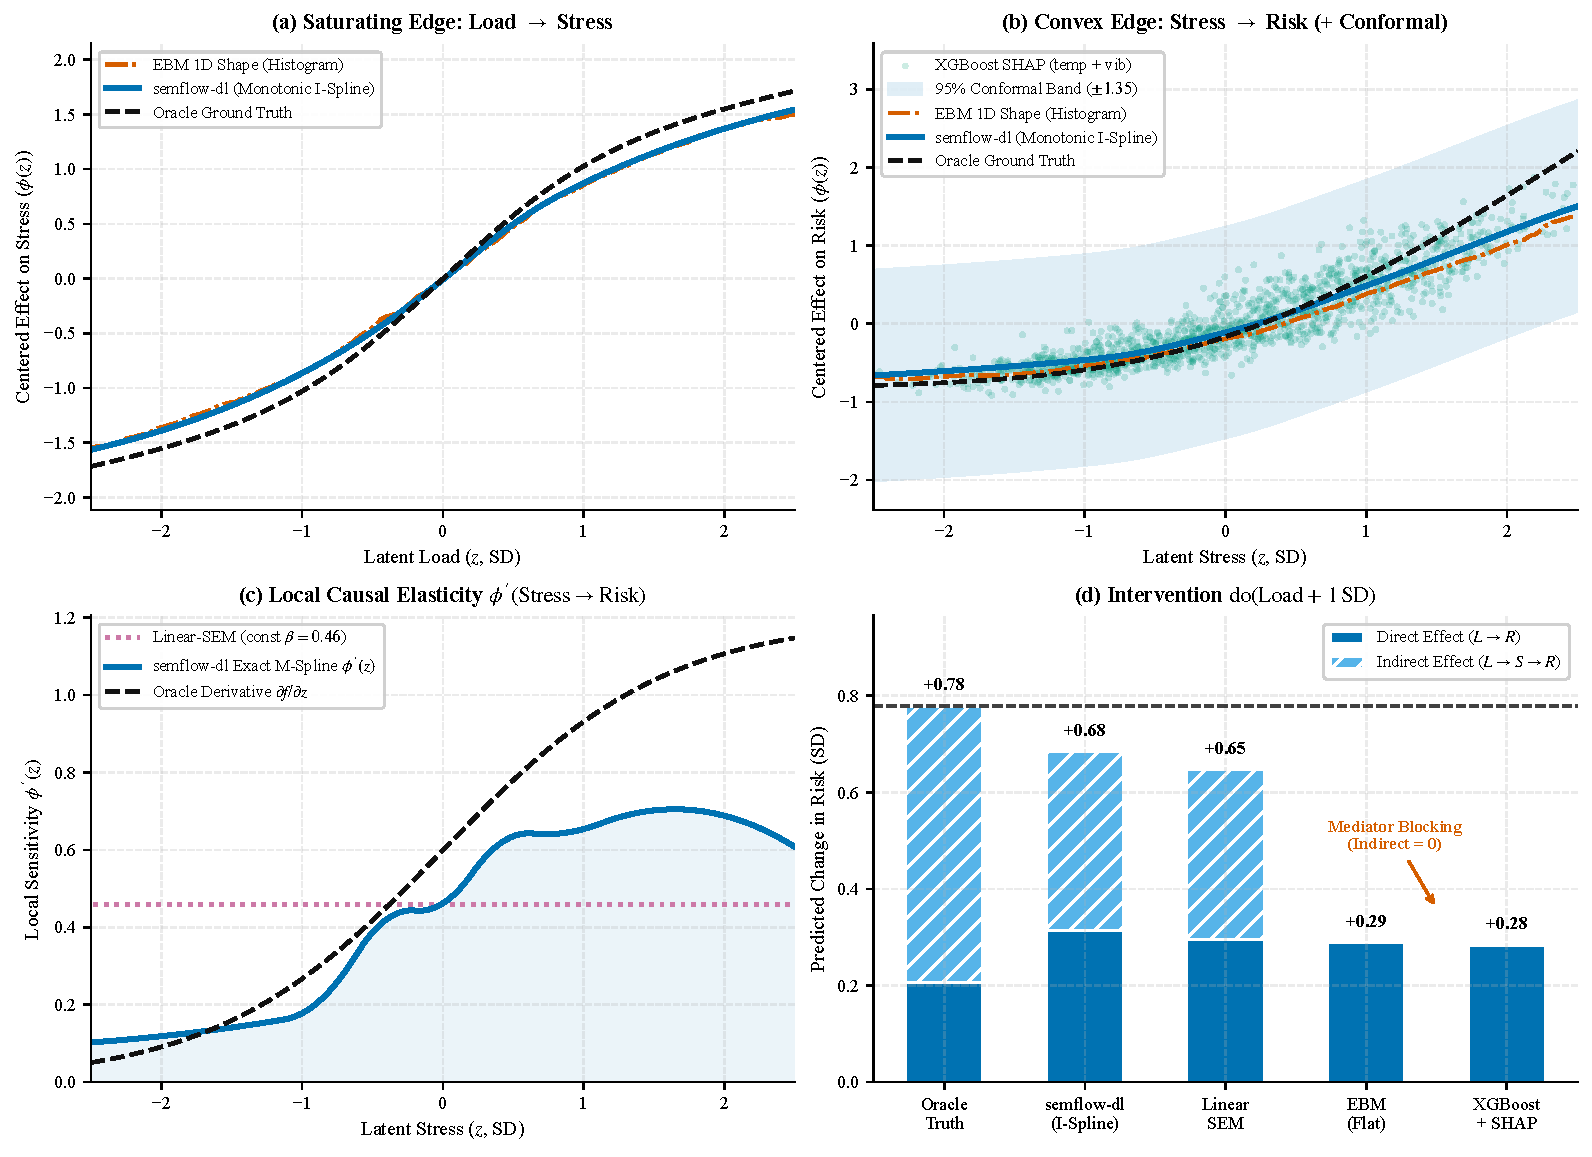
\includegraphics[width=\textwidth]{figures/fig_whitebox_4panel.pdf}
  \caption{Qualitative and causal comparison on the nonlinear mediation benchmark ($\mathrm{Load} \to \mathrm{Stress} \to \mathrm{Risk}$ with noisy dual indicators).
  \textbf{(a)}~Saturating edge recovery ($\mathrm{Load} \to \mathrm{Stress}$): \texttt{semflow-dl} tracks the monotonic ground truth smoothly without histogram binning artifacts.
  \textbf{(b)}~Convex edge recovery ($\mathrm{Stress} \to \mathrm{Risk}$) with 95\% split-conformal prediction bands ($\pm 1.35$\,SD), contrasted against dispersed TreeSHAP attributions and EBM step curves.
  \textbf{(c)}~Closed-form local causal elasticity $\phi'(\mathrm{Stress} \to \mathrm{Risk})$ via M-Spline derivatives, capturing tail-risk acceleration missed by constant-slope Linear-SEM ($\beta = 0.46$).
  \textbf{(d)}~Structural intervention $\mathrm{do}(\mathrm{Load} + 1\,\mathrm{SD})$, illustrating severe mediator blocking ($\mathrm{Indirect} = 0$) in flat EBM and XGBoost+SHAP versus accurate direct--indirect decomposition in \texttt{semflow-dl}.}
  \label{fig:whitebox-4panel}
\end{figure*}

Figure~\ref{fig:whitebox-4panel} visually confirms these quantitative findings. In Panels~(a) and~(b), \texttt{semflow-dl} recovers both the saturating $\mathrm{Load} \to \mathrm{Stress}$ curve and the convex $\mathrm{Stress} \to \mathrm{Risk}$ acceleration smoothly across $[-2.5, +2.5]$\,SD while enclosing test observations within finite-sample 95\% split-conformal bands ($\pm 1.35$\,SD). Panel~(c) highlights a core advantage over both Linear-SEM and flat glass-box models: the exact M-Spline derivative $\phi'(z)$ reveals how marginal risk sensitivity rises from near-zero under low stress to over $0.70$ under high stress, whereas Linear-SEM collapses this regime shift into a single constant slope ($\beta = 0.46$). Finally, Panel~(d) demonstrates why flat models fail under policy simulation: because EBM and XGBoost+SHAP hold the noisy mediator indicators fixed during perturbation, their predicted intervention effects ($+0.29$ and $+0.28$\,SD) miss the entire indirect pathway, whereas \texttt{semflow-dl} ($+0.68$\,SD) closely recovers the oracle total effect ($+0.78$\,SD) and cleanly separates direct and indirect contributions.

\subsection{Wind Turbine SCADA Thermal Stress Case Study}
On a physics-grounded wind-turbine SCADA dataset ($N = 50{,}000$, with $2\%\text{--}4\%$ sensor dropout) modeling $\texttt{Wind} \to \texttt{Load} \to \texttt{Stress} \to \texttt{Loss}$, \texttt{semflow-dl} fits the entire DAG with 95\% split-conformal calibration in $5.0$~s (Table~\ref{tab:scada-case}), decomposing $\mathrm{do}(\mathrm{Load} + 1\,\mathrm{SD})$ on \texttt{Loss} into $+0.2824$ direct and $+0.1838$ indirect effects ($+0.4662$ total), while revealing a $5.6\times$ increase in local thermal elasticity $\phi'(\mathrm{Load} \to \texttt{Stress})$ from low load ($0.087$) to high load ($0.489$).

\begin{table}[t]
  \centering
  \caption{Wind-turbine SCADA thermal stress case study summary ($N = 50{,}000$, 2\%--4\% sensor dropout).}
  \label{tab:scada-case}
  \small
  \begin{tabular}{lll}
    \hline
    Metric / Causal Quantity & \texttt{semflow-dl} (I-Spline + Conformal) & Interpretation \\
    \hline
    Total Fit + Calibration Time & 5.00 s & CPU-only, 95\% Split-Conformal \\
    $\mathrm{do}(\mathrm{Load} + 1\,\mathrm{SD}) \to \mathrm{Loss}$ (Total) & $+0.4662$ SD & Direct $+0.2824$ + Indirect $+0.1838$ \\
    Local Elasticity $\phi'(\mathrm{Load} \to \mathrm{Stress})$ (Low Load) & $0.087$ & Mild thermal sensitivity \\
    Local Elasticity $\phi'(\mathrm{Load} \to \mathrm{Stress})$ (High Load) & $0.489$ & \textbf{5.6$\times$} thermal acceleration regime \\
    \hline
  \end{tabular}
\end{table}

\section{Discussion and Limitations}
\label{sec:discussion}

The empirical results demonstrate that embedding univariate monotonic I-Splines directly onto the edges of an identified latent DAG resolves a fundamental blind spot in contemporary tabular machine learning. Rather than treating interpretability as a post-hoc approximation over black-box ensembles (SHAP) or restricting glass-box models to flat covariate-to-target mappings (EBM, NAM), \texttt{semflow-dl} preserves mechanistic causal structure while retaining nonlinear expressiveness and low-memory CPU efficiency.

Nevertheless, several methodological assumptions and limitations warrant careful consideration:

\begin{enumerate}
  \item \textbf{Specification of the Causal DAG:} Consistent with confirmatory Structural Equation Modeling, \texttt{semflow-dl} assumes that the directed acyclic graph $\mathcal{G}$ and measurement indicator groupings are specified from domain theory or prior causal discovery. Misspecifying edge directions or omitting key mediators will bias the resulting $\mathrm{do}(\cdot)$ decomposition.
  \item \textbf{Unmeasured Confounding:} Proposition~\ref{prop:mediation} relies on the standard structural causal assumption of no unmeasured confounders between parent and child latents ($\mathbb{E}[\zeta_j \mid \mathrm{Pa}(j)] = 0$). In observational settings where latent confounding is suspected, sensitivity analyses or instrumental-variable extensions remain necessary.
  \item \textbf{Measurement Attenuation in Two-Stage Anchoring:} To achieve fast, convex-like convergence without GPU overhead, \texttt{semflow-dl} estimates anchored latent scores via first-principal-component power iteration prior to fitting edge splines. As visible in the slight gap between the estimated curve and the noise-free oracle in Figure~\ref{fig:whitebox-4panel}(a)--(c), finite-indicator measurement error introduces mild residual attenuation. Joint end-to-end latent-and-spline estimation or PLSc-style reliability disattenuation represents a promising direction to further tighten oracle recovery.
  \item \textbf{Exchangeability under Distribution Shift:} While Proposition~\ref{prop:conformal} guarantees distribution-free finite-sample coverage on exchangeable test sets, non-stationary time-series telemetry (such as seasonal wind-turbine regimes) can violate exchangeability. Extending the current split-conformal calibrator to Adaptive Conformal Inference (ACI) and integrating the sparse CSR spatial coupling module ($\rho\mathbf{W}$) into streaming edge deployments are immediate priorities for future releases.
\end{enumerate}

\section{Conclusion}
\label{sec:conclusion}

We introduced \texttt{semflow-dl}, a pure-Rust edge-level white-box causal deep learning library with zero-copy Python bindings designed as a modular extension to the \texttt{semflow} ecosystem. By combining anchored latent measurement models, Ramsay's monotonic I-Spline edge operators, ANOVA-purified 2D interactions, exact Pearl counterfactual propagation, and split-conformal calibration, \texttt{semflow-dl} bridges the gap between classical linear SEM and modern tabular machine learning. Across controlled mediation benchmarks and a wind-turbine SCADA case study, \texttt{semflow-dl} reduces causal intervention error by more than $5\times$ compared to EBM and XGBoost+SHAP, guarantees $0.0\%$ monotonicity violations, provides closed-form local causal elasticity via M-Spline derivatives, and operates within 87\,MB of RAM on standard CPU hardware. All source code, parity tests, and reproducible benchmark scripts are openly available to support transparent, causally grounded modeling across scientific and engineering disciplines.


\bibliographystyle{plainnat}
\bibliography{references}

\end{document}
